\chapter{Arhitektura i dizajn sustava}
		Arhitektura sustava počiva na podjeli na korisničko sučelje \textit{(en. frontend)} i na pozadinsku aplikaciju \textit{(en. backend)} koja se spaja na relacijsku bazu podataka.

		Glavna tehnologija izrade "frontend" dijela sustava je React.js razvojni okvir, a samo korisničko sučelje je izgrađeno od gotovih komponenti iz paketa "Bootstrap". Korištenje Bootstrap-a omogućuje brzo i lako razvijanje sučelja koja izgledaju moderno i koja su responzivna, 
		što je jedan od važnijih zahtjeva. 

		Backend dio je izrađen u Spring radnom okviru koji omogućava razvoj MVC (Model-View-Controller) aplikacija, ali i još puno toga, poput rada s bazama podataka i autorizacije korisnika (Spring Security). 
		Za postavljanje aplikacije u skladu sa Springovim konvencijama koristili smo Spring Boot ekstenziju.

		Kao relacijsku bazu podataka odabrali smo Postgres. Radi se o bazi otvorenog koda \textit{(en. open-source)} visokih performansi koja se koristi za širok raspon zadataka i u raznim okruženjima.

		\begin{figure}[H]
			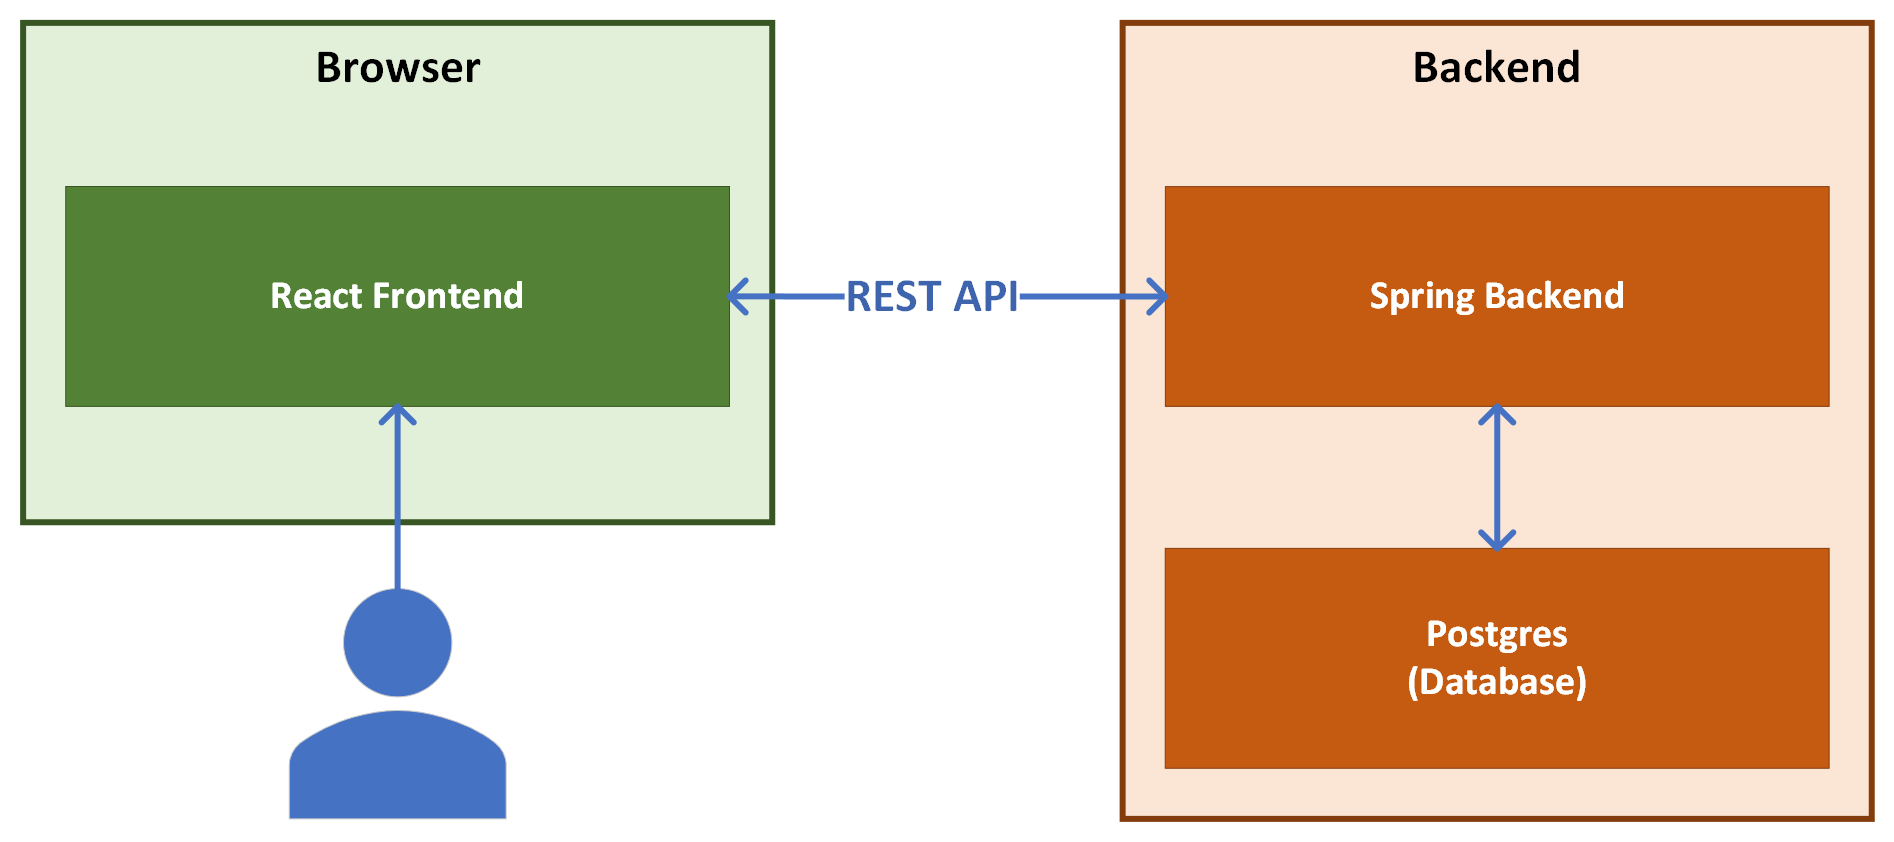
\includegraphics[width=\textwidth]{slike/architecture.png} 
			\caption{Dijagram arhitekture sustava "Ozdravi".}
			% \label{fig:promjene2} 
		\end{figure}

		Kao što je prikazano na slici 4.1, središnji je dio sustava Spring backend koji ostvaruje komunikaciju s Postgres bazom, ali i s frontend aplikacijom. Komunikacija s frontend-om se ostvaruje primjenom
		HTTP (HyperText Transfer Protokola) protokola koji je ključni protokol web-a. Za potrebe komunikacije backend-a i frontend-a definiran je API (Application Programming Interface) u skladu s pravilima REST-a (Representational State Transfer). Neka od njih su:
		\begin{packed_item}
			\item odvajanje poslužitelja i klijenta - klijent i poslužitelj su u potpunosti neovisni, a sve što klijent "zna" dolazi od poslužitelja
			\item "statelessness" - zahtjevi klijenta prema poslužitelju su međusobno neovisni i sadrže sve informacije potrebne za svoje izvođenje
		\end{packed_item}

		U kontekstu Spring razvojnog okvira, aplikacija koristi tri arhitekturna sloja (Controller, Service i Repository) kako bi se organizirao kod i razdvojile odgovornosti:
		\begin{packed_item}
			\item Controller - Sloj koji obrađuje HTTP zahtjeve i upravlja komunikacijom između korisničkog sučelja (frontend) i ostatka aplikacije. Kontroleri su odgovorni za prihvat HTTP zahtjeva, obradu korisničkih ulaznih podataka, pozivanje odgovarajućih metoda u Service sloju i pripremu odgovora za korisnika.		
			\item Service - Sloj koji sadrži poslovnu logiku aplikacije. Servisi se koriste kako bi se odvojila poslovna logika od kontrolera i omogućila ponovna upotreba iste logike na različitim dijelovima aplikacije.
			\item Repository - Sloj koji je odgovoran za pristup podacima. To uključuje komunikaciju s bazom podataka. Repository sloj omogućava izvršavanje osnovnih operacija poput spremanja, dohvaćanja, ažuriranja i brisanja podataka.
		\end{packed_item}
    
		Zahtjevi prema backendu dolaze iz React aplikacije koja se izvršava unutar korisničkog preglednika, a ne na nekom vanjskom poslužitelju. Ipak, kako bi ju pokrenuo, korisnički preglednik tu aplikaciju mora preuzeti od negdje. To je prikazano na slici 4.2. 

		\begin{figure}[H]
			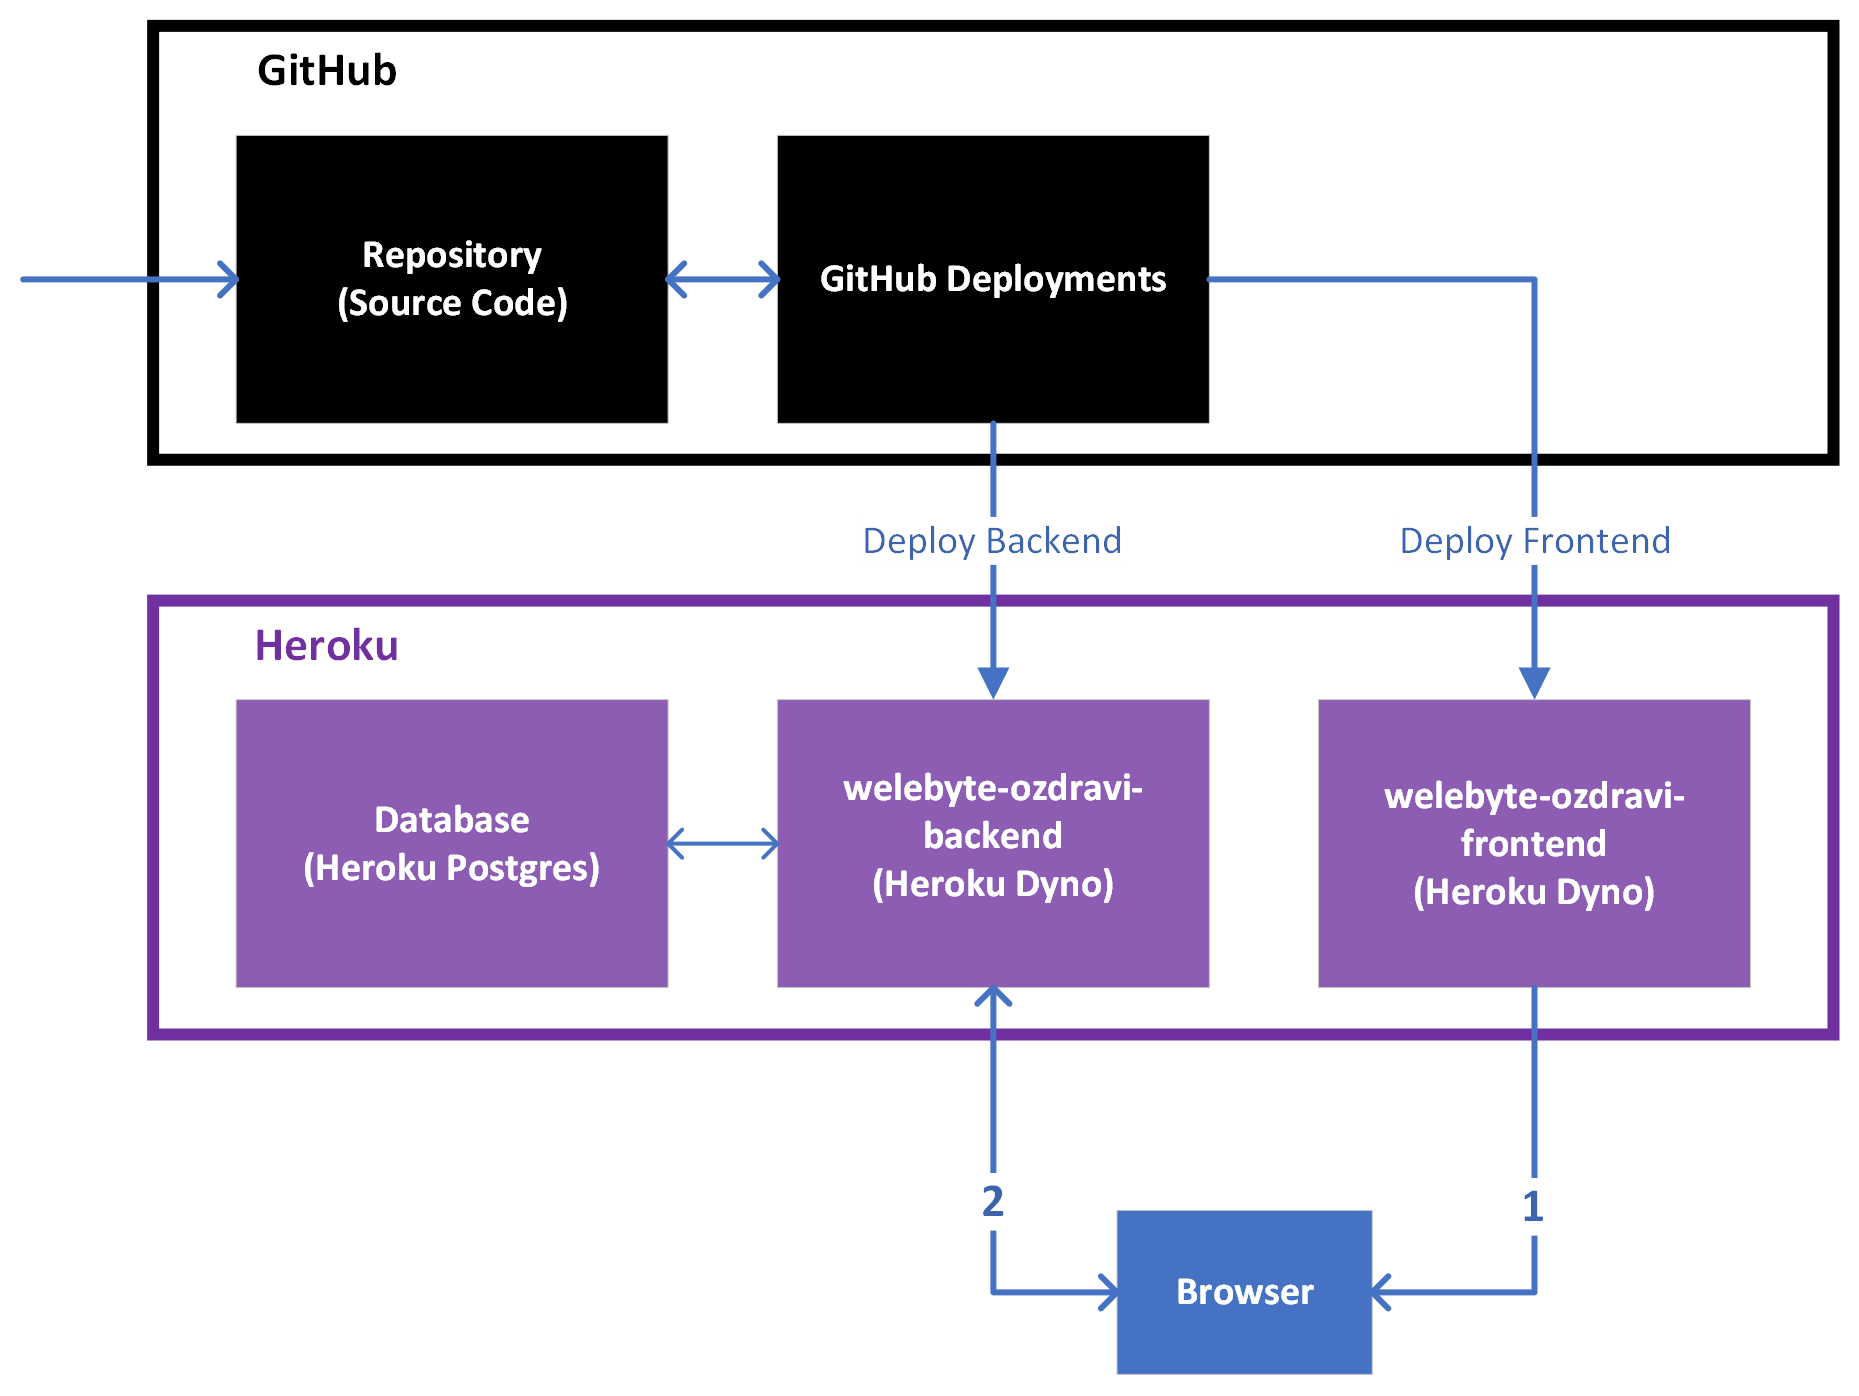
\includegraphics[width=\textwidth]{slike/infrastructure.png} 
			\caption{Dijagram infrastrukture sustava "Ozdravi".}
		\end{figure}

		U produkcijskom okruženju, sustav koristi dva poslužitelja - jedan pokreće Spring aplikaciju (backend), a drugi omogućava preglednicima preuzimanje React aplikacije (frontend).

		Kao infrastrukturnu platformu, na kojoj ćemo postaviti produkcijsko okruženje, izabrali smo Heroku zbog ova tri razloga:
		\begin{packed_item}
			\item jednostavnost postavljanja potrebnih resursa (Heroku Dyno, Heroku Postgres)
			\item fleksibilan model naplate koji omogućava besplatno korištenje platforme
			\item jednostavno integriranje s GitHub repozitorijem za lagan "deployment" kad je to potrebno
		\end{packed_item}

		Korisnici se u sustav prijavljuju unoseći svoje korisničko ime i lozinku. Na temelju tih vjerodajnica, a nakon provjere s podacima u bazi, backend korisniku izdaje token koji se koristi za autentikaciju narednih zahtjeva s klijenta.
		Koristimo "Bearer" autentikacijsku schemu koja podrazumijeva da svaki HTTP zahtjev koji dolazi od klijenta ima token u ispravnom polju u zaglavlju. Ovakva implementacija podrazumijeva korištenje HTTPS protokola koji omogućava komunikaciju na siguran način.
					
		\section{Baza podataka}
        Baza podataka koja se koristi u projektu "Ozdravi" ključna je komponenta sustava koja omogućava pohranu, upravljanje i praćenje svih relevantnih informacija o korisnicima i njihovim zdravstvenim podacima. 
		Izgrađena je relacijska baza podataka koja se sastoji od sljedećih entiteta:
		\begin{packed_item}
			\item Person
			\item Examination
			\item SecondOpinion
			\item Instruction
			\item SickLeaveRecommendation
			\item Address
			\item Role
			\item PersonRoles
		\end{packed_item}

        Baza podataka "Ozdravi" omogućava integraciju svih informacija kako bi podržala procese komunikacije, pregleda i dijagnoza u kontekstu brige o zdravstvenim potrebama djece. Ova struktura omogućava učinkovito praćenje i upravljanje svim 
		relevantnim medicinskim podacima i podržava glavne funkcionalnosti sustava.
        
		\subsection{Opis tablica}

		\textbf{Osoba} Ovaj entitet sadržava osnovne informacije o svim korisnicima sustava, uključujući njihovu ulogu, identifikacijske brojeve, ime, prezime, korisničko ime i lozinku. Ova tablica je ključna za autentikaciju korisnika i definira njihove uloge unutar sustava.
		\begin{longtblr}[
			label=none,
			entry=none
			]{
				width = \textwidth,
				colspec={|X[6,l]|X[6, l]|X[20, l]|}, 
				rowhead = 1,
			} %definicija širine tablice, širine stupaca, poravnanje i broja redaka naslova tablice
			\hline \SetCell[c=3]{c}{\textbf{Person (osoba)}}	 \\ \hline[3pt]
			\SetCell{LightGreen}id & INT	&  	jedinstveni brojčani identifikator 	\\ \hline
			\SetCell{LightBlue}parent\_id	& INT & ID osobe koja je roditelj osobe [Parent] \\ \hline 
			\SetCell{LightBlue}doctor\_id	& INT & ID osobe koja je doktor osobe [Doctor/Pediatrician] \\ \hline 
			\SetCell{LightBlue}address\_id	& INT & ID Adrese osobe \\ \hline 
			OIB & VARCHAR & Osobni identifikacijski broj \\ \hline 
			first\_name & VARCHAR &  Ime osobe (NOT NULL) \\ \hline 
			last\_name & VARCHAR &  Prezime osobe (NOT NULL) \\ \hline 
			role & VARCHAR &  Uloga korisnika (NOT NULL) \\ \hline 
			password & VARCHAR &  Lozinka za prijavu u sustav \\ \hline
			email & VARCHAR &  e-mail za prijavu u sustav \\ \hline 
		\end{longtblr}

		\textbf{Pregled} Ovaj entitet sadržava podatke o pacijentima, uključujući informacije o njihovim pregledima, dijagnozama i zapisnicima. Sadrži atribute: identifikator pregleda, identifikator pacijenta, identifikator liječnika, identifikator liječnika koji je zakazao pregled, identifikator adrese na kojoj se održava pregled, zapisnik s pregleda te datum i vrijeme pregleda. Pohranjuje veze između pacijenata, doktora i pregleda, omogućavajući praćenje medicinskih podataka. 
		
		\begin{longtblr}[
			label=none,
			entry=none
			]{
				width = \textwidth,
				colspec={|X[6,l]|X[6, l]|X[20, l]|}, 
				rowhead = 1,
			} 
			\hline \SetCell[c=3]{c}{\textbf{Examination (Pregled)}}	 \\ \hline[3pt]
			\SetCell{LightGreen}id & INT	&  	jedinstveni brojčani identifikator 	\\ \hline
			\SetCell{LightBlue}patient\_id	& INT & ID osobe koja je pacijent [Parent/Child] (NOT NULL) \\ \hline 
			\SetCell{LightBlue}doctor\_id	& INT & ID osobe koja vrši pregled [Doctor/Pediatrician] (NOT NULL) \\ \hline 
			\SetCell{LightBlue}scheduler\_id	& INT & ID osobe koja je zakazala pregled [Doctor/Pediatriciran] (NOT NULL) \\ \hline 
			\SetCell{LightBlue}address\_id	& INT & ID adrese na kojoj se održava pregled \\ \hline 
			report & TEXT & Dijagnoza/zapisnik s pregleda \\ \hline 
			date & DATETIME &  Datum i vrijeme pregleda (NOT NULL) \\ \hline 
		\end{longtblr}

		\textbf{Drugo mišljenje} Ovaj entitet služi za praćenje detalja o pregledima pacijenata. Sadrži atribute: identifikator drugog mišljenja, identifikator osobe koja ga je zatražila, identifikator liječnika koji daje drugo mišljenje te nalaz iz privatne ustanove na temelju kojeg se traži drugo mišljenje. Ovaj entitet omogućava praćenje medicinskih konzultacija.
		\begin{longtblr}[
			label=none,
			entry=none
			]{
				width = \textwidth,
				colspec={|X[6,l]|X[6, l]|X[20, l]|}, 
				rowhead = 1,
			} 
			\hline \SetCell[c=3]{c}{\textbf{SecondOpinion (DrugoMišljenje)}}	 \\ \hline[3pt]
			\SetCell{LightGreen}id & INT	&  	jedinstveni brojčani identifikator 	\\ \hline
			\SetCell{LightBlue}requester\_id	& INT & ID osobe koja je zatražila drugo mišljenje [Parent] (NOT NULL) \\ \hline 
			\SetCell{LightBlue}doctor\_id & INT & ID osobe koja je dala drugo mišljenje [Doctor/Pediatrician] (NOT NULL) \\ \hline 
			private\_report & TEXT & nalaz iz privatne ustanove koji unosi roditelj (NOT NULL)\\ \hline 
			content & TEXT &  Sadržaj na koji se daje drugo mišljenje (nalaz iz privatne ustanove) \\ \hline 
		\end{longtblr}

		\textbf{Uputa} Ovaj entitet sadržava informacije o izdanim uputama, uključujući informacije o pacijentima, doktorima koji stvaraju upute i statusu upute. Sadrži atribute: identifikator upute, identifikator liječnika koji je izdao uputu, identifikator pacijenta kojemu je upućena, datum te sadržaj upute. Omogućava praćenje i upravljanje medicinskim preporukama.
		\begin{longtblr}[
			label=none,
			entry=none
			]{
				width = \textwidth,
				colspec={|X[6,l]|X[6, l]|X[20, l]|}, 
				rowhead = 1,
			} 
			\hline \SetCell[c=3]{c}{\textbf{Instruction (Uputa)}}	 \\ \hline[3pt]
			\SetCell{LightGreen}id & INT	&  	jedinstveni brojčani identifikator 	\\ \hline
			\SetCell{LightBlue}doctor\_id	& INT & ID osobe koja je izdala uputu [Doctor/Pediatrician] (NOT NULL) \\ \hline 
			\SetCell{LightBlue}patient\_id & INT & ID osobe za koju je uputa [Parent] (NOT NULL) \\ \hline 
			date & DATETIME & Datum i vrijeme izdavanja upute (NOT NULL)\\ \hline 
			content & TEXT &  Sadržaj upute (NOT NULL) \\ \hline 
		\end{longtblr}

\textbf{Preporuka za bolovanje} Ovaj entitet sadržava informacije o izdanim preporukama za bolovanje, tko ih je izdao, za koga i tko ih treba odobriti. Sadrži atribute: identifikator preporuke, identifikator pacijenta, identifikator pedijatra koji ju je stvorio, identifikatora liječnika koji ju je odobrio, identifikator pregleda na kojem se izdaje te status preporuke.
		\begin{longtblr}[
			label=none,
			entry=none
			]{
				width = \textwidth,
				colspec={|X[6,l]|X[6, l]|X[20, l]|}, 
				rowhead = 1,
			} 
			\hline \SetCell[c=3]{c}{\textbf{SickLeaveRecommendation (Preporuka za bolovanje)}}	 \\ \hline[3pt]
			\SetCell{LightGreen}id & INT	&  	jedinstveni brojčani identifikator	\\ \hline
			\SetCell{LightBlue}patient\_id & INT & ID osobe za koju se traži bolovanje [Parent] (NOT NULL) \\ \hline 
			\SetCell{LightBlue}creator\_id & INT & ID osobe koja je stvorila preporuku [Pediatrician] (NOT NULL) \\ \hline
			\SetCell{LightBlue}approver\_id & INT & ID osobe koja mora odobriti preporuku [Doctor] (NOT NULL) \\ \hline 
			\SetCell{LightBlue}examination\_id	& INT & ID pregleda na temelju kojeg se izdaje preporuka (NOT NULL) \\ \hline 
			status & BOOLEAN &  Je li preporuka odobrena? (default false) \\ \hline 
		\end{longtblr}

        \textbf{Adresa} Ovaj entitet sadržava informacije o adresi održavanja pregleda. Sadrži atribute: identifikator ulice, ulicu, kućni broj, grad, državu te geografsku širinu i dužinu. 
		\begin{longtblr}[
			label=none,
			entry=none
			]{
				width = \textwidth,
				colspec={|X[6,l]|X[6, l]|X[20, l]|}, 
				rowhead = 1,
			} 
			\hline \SetCell[c=3]{c}{\textbf{Address (Adresa)}}	 \\ \hline[3pt]
			\SetCell{LightGreen}id & INT	&  	jedinstveni brojčani identifikator 	\\ \hline
			street	& VARCHAR & ulica\\ \hline 
            number	& VARCHAR & kućni broj\\ \hline
            city	& VARCHAR & grad\\ \hline
            country	& VARCHAR & država\\ \hline
            latitude	& NUMERIC & geografska širina\\ \hline
            longitude	& NUMERIC & geografska dužina\\ \hline
			
		\end{longtblr}

		\textbf{Uloga} Ovaj entitet sadržava informacije o mogućim ulogama u sustavu. Sadrži atribute: identifikator uloge i naziv uloge. 
		\begin{longtblr}[
			label=none,
			entry=none
			]{
				width = \textwidth,
				colspec={|X[6,l]|X[6, l]|X[20, l]|}, 
				rowhead = 1,
			} 
			\hline \SetCell[c=3]{c}{\textbf{Role (Uloga)}}	 \\ \hline[3pt]
			\SetCell{LightGreen}id & INT	&  	jedinstveni brojčani identifikator 	\\ \hline
			\SetCell{LightBlue}name	& VARCHAR & naziv uloge\\ \hline 
        
		\end{longtblr}

		\textbf{PersonRoles} Ovaj entitet sadržava informacije o ulogama korisnika u sustavu. Prikazuje koji korisnik ima koju ulogu. Sadrži atribute: identifikator, identifikator uloge i naziv uloge. 
		\begin{longtblr}[
			label=none,
			entry=none
			]{
				width = \textwidth,
				colspec={|X[6,l]|X[6, l]|X[20, l]|}, 
				rowhead = 1,
			} 
			\hline \SetCell[c=3]{c}{\textbf{PersonRoles}}	 \\ \hline[3pt]
			\SetCell{LightGreen}id & INT	&  	jedinstveni brojčani identifikator 	\\ \hline
			\SetCell{LightBlue}role\_id	& VARCHAR & identifikator uloge\\ \hline 
			\SetCell{LightBlue}person\_id	& VARCHAR & identifikator osobe\\ \hline
        
		\end{longtblr}
  
		\subsection{Dijagram baze podataka}
			% U ovom potpoglavlju potrebno je umetnuti dijagram baze podataka. Primarni i strani ključevi moraju biti označeni, a tablice povezane. Bazu podataka je potrebno normalizirati.
		    \begin{figure}[H]
			     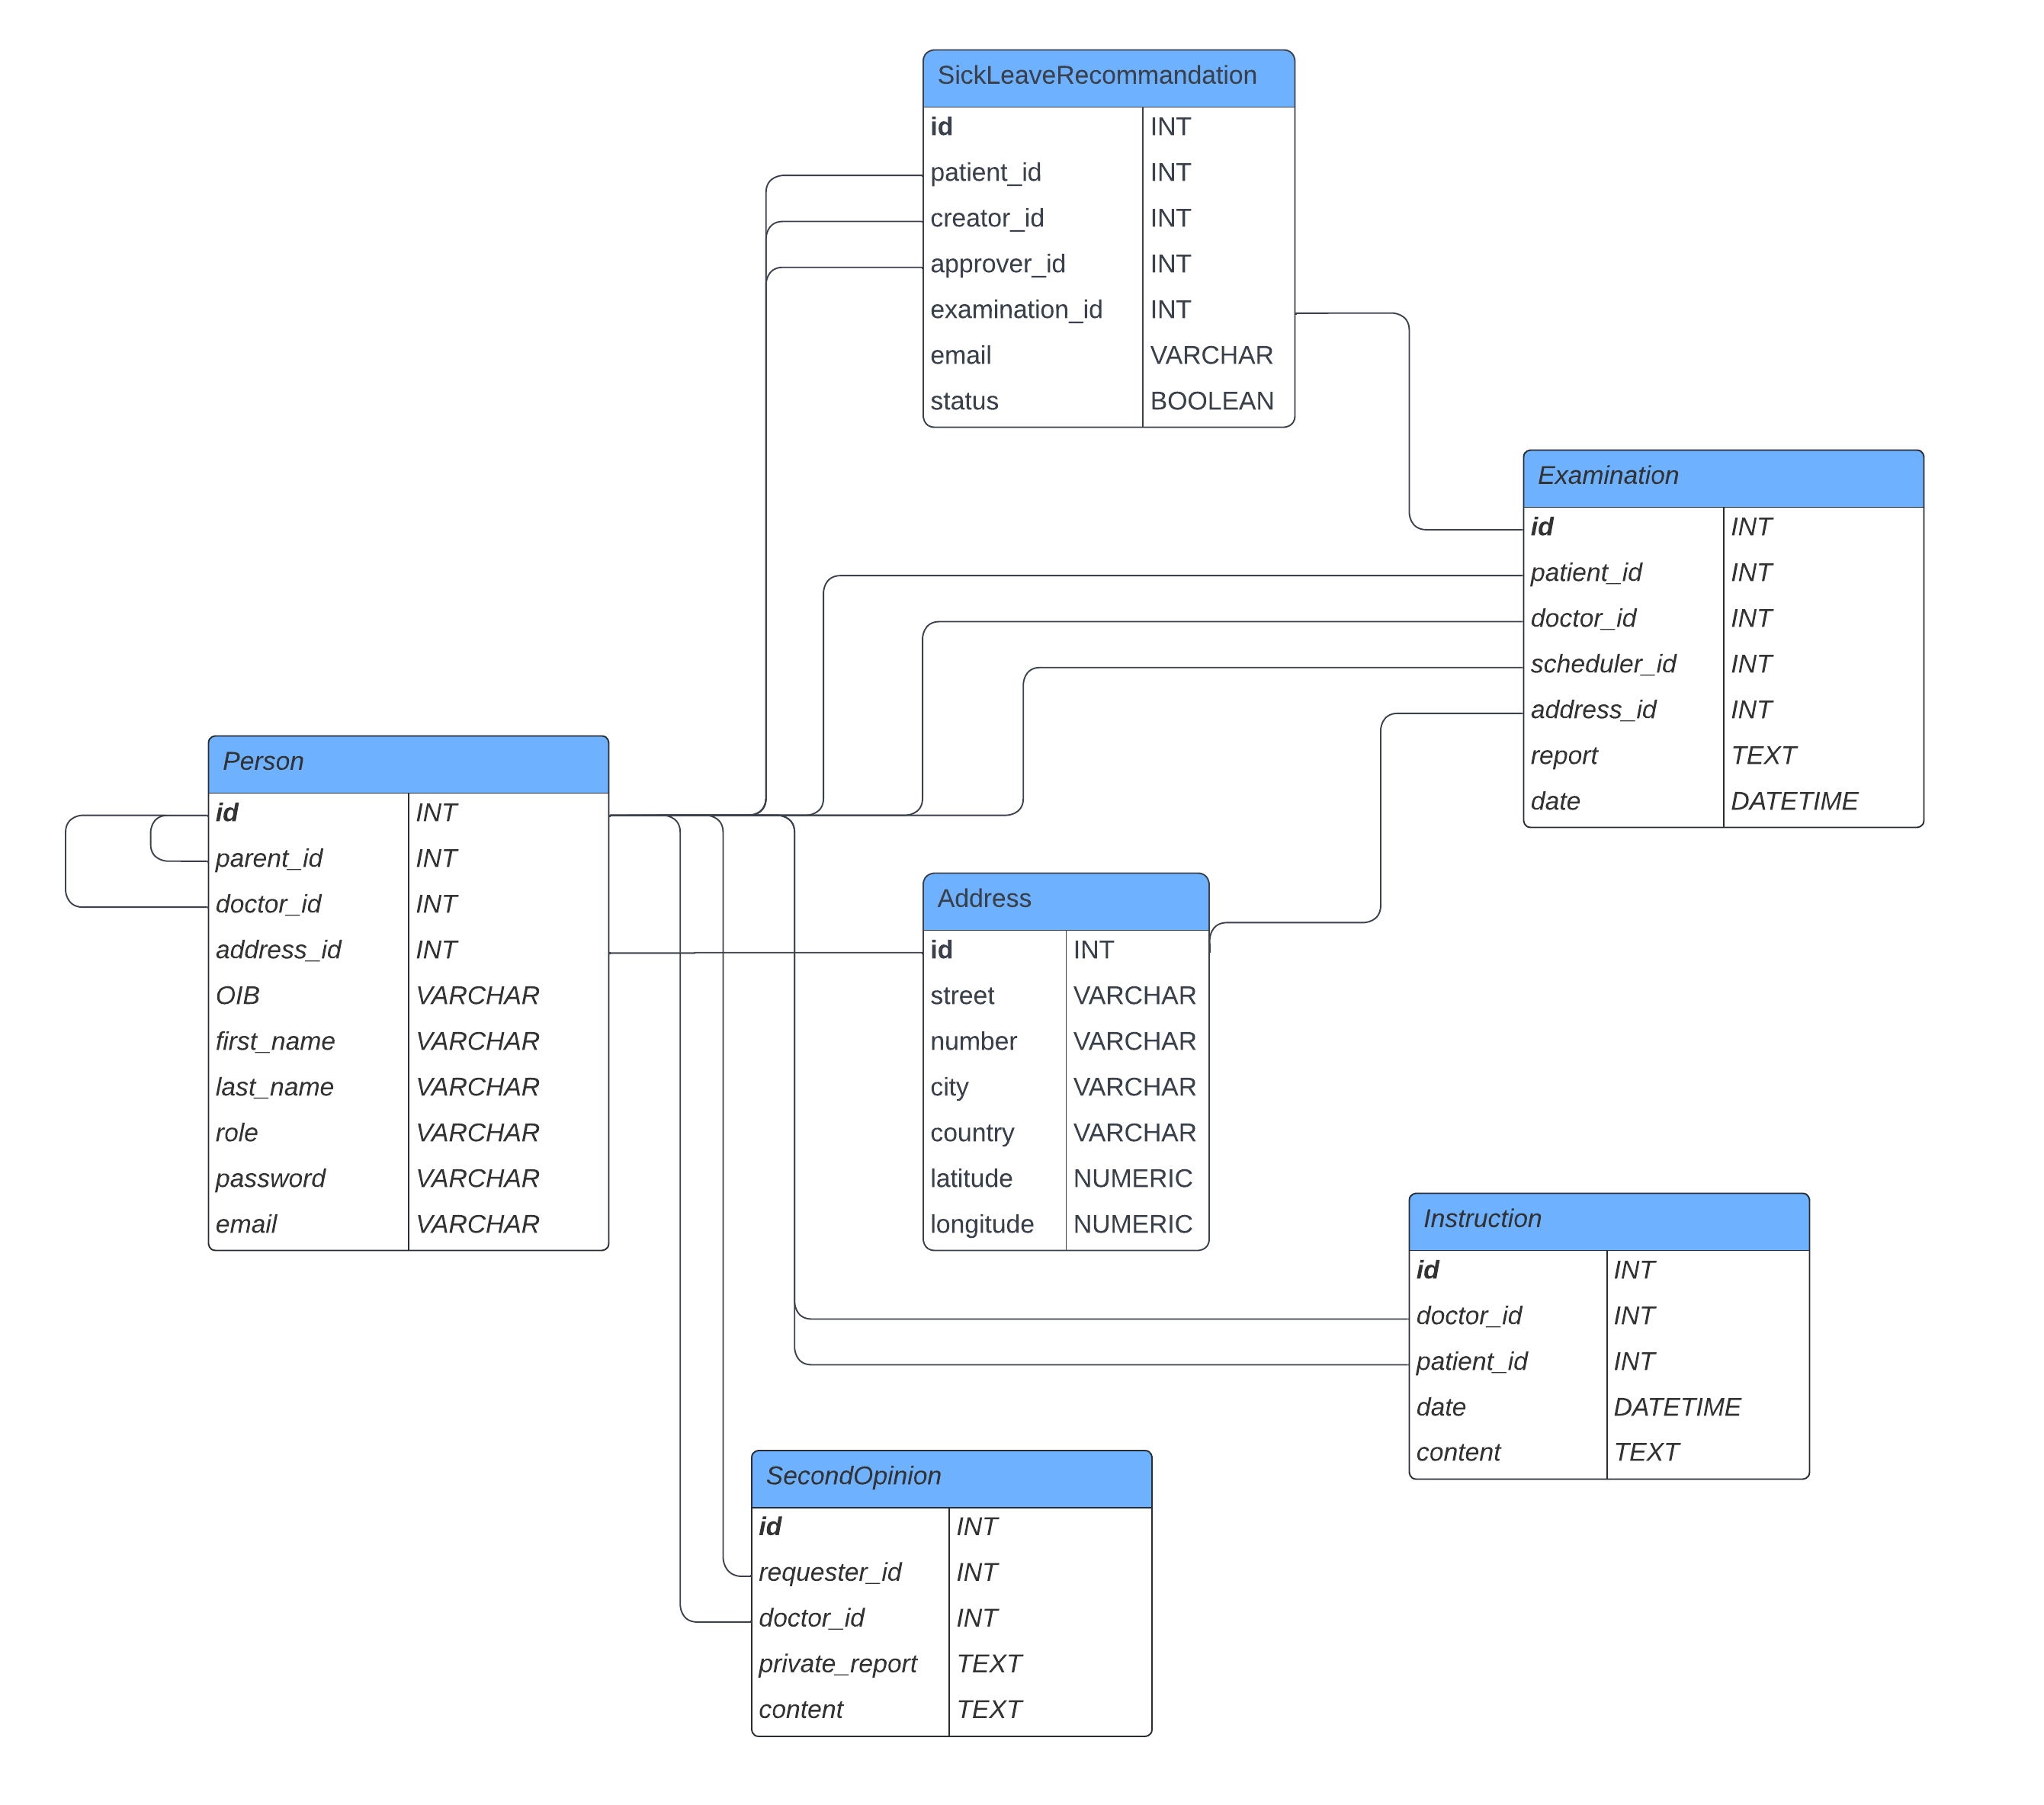
\includegraphics[width=\textwidth]{slike/DijagramBazePodataka.png} 
			     \caption{ER dijagram baze podataka} 
		    \end{figure}
		\eject
		
			
		\section{Dijagram razreda}
		
			%Potrebno je priložiti dijagram razreda s pripadajućim opisom. Zbog preglednosti je moguće dijagram razlomiti na više njih, ali moraju biti grupirani prema sličnim razinama apstrakcije i srodnim funkcionalnostima.
			
			%dio 1. revizije
			
			%Prilikom prve predaje projekta, potrebno je priložiti potpuno razrađen dijagram razreda vezan uz generičku funkcionalnost sustava. Ostale funkcionalnosti trebaju biti idejno razrađene u dijagramu sa sljedećim komponentama: nazivi razreda, nazivi metoda i vrste pristupa metodama (npr. javni, zaštićeni), nazivi atributa razreda, veze i odnosi između razreda.
			
			%dio 2. revizije			
			
			%Prilikom druge predaje projekta dijagram razreda i opisi moraju odgovarati stvarnom stanju implementacije
			
			
			
			\eject
		
		\section{Dijagram stanja}
			
			
			%dio 2. revizije
			
			%Potrebno je priložiti dijagram stanja i opisati ga. Dovoljan je jedan dijagram stanja koji prikazuje značajan dio funkcionalnosti sustava. Na primjer, stanja korisničkog sučelja i tijek korištenja neke ključne funkcionalnosti jesu značajan dio sustava, a registracija i prijava nisu.
			
			
			\eject 
		
		\section{Dijagram aktivnosti}
			
			%dio 2. revizije
			
			 %Potrebno je priložiti dijagram aktivnosti s pripadajućim opisom. Dijagram aktivnosti treba prikazivati značajan dio sustava.
			
			\eject
		\section{Dijagram komponenti}
		
			%dio 2. revizije
		
			 %Potrebno je priložiti dijagram komponenti s pripadajućim opisom. Dijagram komponenti treba prikazivati strukturu cijele aplikacije.